% vim: set tw=0:
\documentclass{beamer}
\usepackage{graphicx}

% Reasonable themes:
% Antibes Bergen Berkeley Berlin Frankfurt Goettingen Ilmenau Luebeck Malmoe
% Montpellier PaloAlto Rochester Singapore Szeged Warsaw bars boxes
% compatibility default lined plain shadow sidebar split tree
% And these ones include the author's name on every slide:
% Berkeley

% Declare themes.
\mode<presentation>
\usetheme{UWHEP}

% Personal macros.
\newcommand{\email}[1]{{\texttt #1}}
\newcommand{\newframe}[1]{\section{#1}
    \frametitle{\sc{#1}}}
\newcommand{\subframe}[1]{\subsection{#1}
    \frametitle{\sc{#1}}}
\newcommand{\supers}[1]{\ensuremath{^\textrm{#1}}}
\newcommand{\subs}[1]{\ensuremath{_\textrm{#1}}}
\newcommand{\ca}{\ensuremath{\sim}}

% Author information.
\title{T2 Status}
\author[Maier, Mohapatra]{
    Will Maier \and Ajit Mohapatra\\ 
    {\tt wcmaier@hep.wisc.edu}\\
    {\tt ajit@hep.wisc.edu}}
\institute[Wisconsin]{University of Wisconsin - High Energy Physics}
\date{\today}
\logo{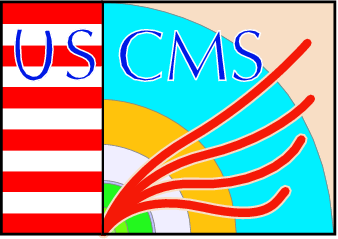
\includegraphics[height=0.6cm]{../../../Graphics/USCMS_logo.png}\hspace{.1cm}
\includegraphics[height=0.75cm]{../../../Graphics/UW_logo.png}}

\begin{document}

\begin{frame}
    \titlepage
\end{frame}

%\section{Overview}
%\begin{frame}
%    \tableofcontents
%\end{frame}

\section{Facilities}
\subsection{Software and Storage}
\begin{frame}
\frametitle{}
\begin{itemize}
    \item CRAB jobs are hammering AFS
    \begin{itemize}
        \item Untar payload before {\tt chdir()} into scratch space
        \item Sent patch upstream, but other jobs still violate assumptions
        \item Deploying parts of NFSlite to minimize use of AFS
        \item Also discovered that gatekeeper wasn't fully using local wnclient installation -- still debugging
        \item gatekeeper on- and offline today
    \end{itemize}
    \item Switched to new edge router and fiber path
    \begin{itemize}
        \item Due to planned construction, old router was being decommissioned
        \item Now on new router with lower load
        \item New router also has access to more fiber -- campus says we can provision new bandwidth dynamically/temporarily
        \item Should be suitable for burst traffic
    \end{itemize}
\end{itemize}
\end{frame}

\subsection{Production and Monitoring}
\begin{frame}
\frametitle{}
\begin{itemize}
    \item SAM: OK
    \begin{itemize}
        \item Good until today (gatekeeper problems)
    \end{itemize}
    \item JobRobot: OK 
    \item PhEDEx:
    \begin{itemize}
        \item DDT2 link exercises in Prod (CNAF, ASGC, CERN, FNAL) last week -- most transfers OK
        \item MC data subscriptions for local users
    \end{itemize}
    \item MC Production:
    \begin{itemize}
        \item CSA08 preproduction is over
        \item (In)famous MadGraph production ran last week (causing all sorts of pain and suffering to the OSG T2s), but it's over
        \item Skim jobs will run over this DS starting from tomorrow
    \end{itemize}
\end{itemize}
\end{frame}

\end{document}
